\section{Related Work}\label{sec:related}


In recent years, one of the key technologies in remote sensing is hyperspectral imaging and associated anomaly detection (HAD). It is frequently employed in both military and civilian domains because of its feature. However, because of environmental light variations, interference like atmospheric scattering, the mixed pixel problem brought on by low spatial resolution, and the absence of anomaly sample labels~\cite{keshava2002spectral,shi2014incorporating,nishii1996enhancement}, HAD currently depends on the statistical characteristics of the data itself or deep features to distinguish the background from the anomaly. Model-based approaches~\cite{schweizer_efficient_2001} and deep learning-based methods~\cite{schweizer_efficient_2001,chang2007hyperspectral,li_learning_2024,Cui2024Semi} are the two main classes of HAD techniques.


\subsection{Traditional Methods}

Model-driven anomaly detection techniques, which primarily consist of two primary algorithmic frameworks, statistical modeling and representation learning—dominate classical HAD research~\cite{su2021hyperspectral}. Reed introduced statistical HAD with the Reed-Xiaoli (RX) approach, which makes the assumption that the background follows a multivariate Gaussian distribution and that Mahalanobis distance thresholding is used to identify the anomalies~\cite{RXD,su2021hyperspectral}. A number of variations have been created to improve robustness, such as Kernel-RX (KRX)~\cite{su2021hyperspectral,kwon2005kernel}, Local-RX (LRX)~\cite{su2021hyperspectral,matteoli2010local}, Segmented-RX~\cite{su2021hyperspectral,matteoli2010improved} and Weighted-RX~\cite{su2021hyperspectral,guo2014weighted}. However, modeling the background distribution with a Gaussian distribution~\cite{matteoli2010tutorial,yang_compressive_2015,manolakis2001statistics} is insufficient due to the intricacy of HSI. 

Over time, representation learning-based detection frameworks have emerged as a research hotspot in an effort to overcome the reliance of conventional HAD techniques on data distribution assumptions. Such methods extract essential features of the data by constructing adaptive representation models. Among them, the widely used ones are low rank representation (LRR)~\cite{gao2021using,zhuang2021hyperspectral,zhuang2020hyperspectral,yin2015laplacian}, collaborative representation (CR)~\cite{zhao2022hyperspectral} and sparse representation (SR)~\cite{zhuang2021fasthymix,li2020lowrank,zhuang2023crosstrack,du_beyond_2016}. In order to mine the spatial-spectral correlation of hyperspectral data from a global perspective, low-rank representation (LRR)~\cite{liu2010robust} models interpixel correlations based on global low-rank constraints, separating anomalies by residuals of the original image from the low-rank background. The collaborative representation detector (CRD)~\cite{zhang2014hyperspectral}, which is based on the a priori assumption that anomalies are hard to represent linearly by neighbors, uses linear combinations of spatial neighborhood pixels to represent the current pixel and detects anomalies using the representation residuals. Nevertheless, the model-driven representation learning approach still has substantial drawbacks~\cite{bioucas2013hyperspectral}: the model hyperparameters (\textit{e.g.,} sparsity, rank constraints) must be manually adjusted, and the parameter settings are highly correlated with the scene; it is also not generalizable, and it is challenging to transfer to other sensors or feature type data once the model has been trained for a particular image.

\begin{figure*}[htbp]
    \centering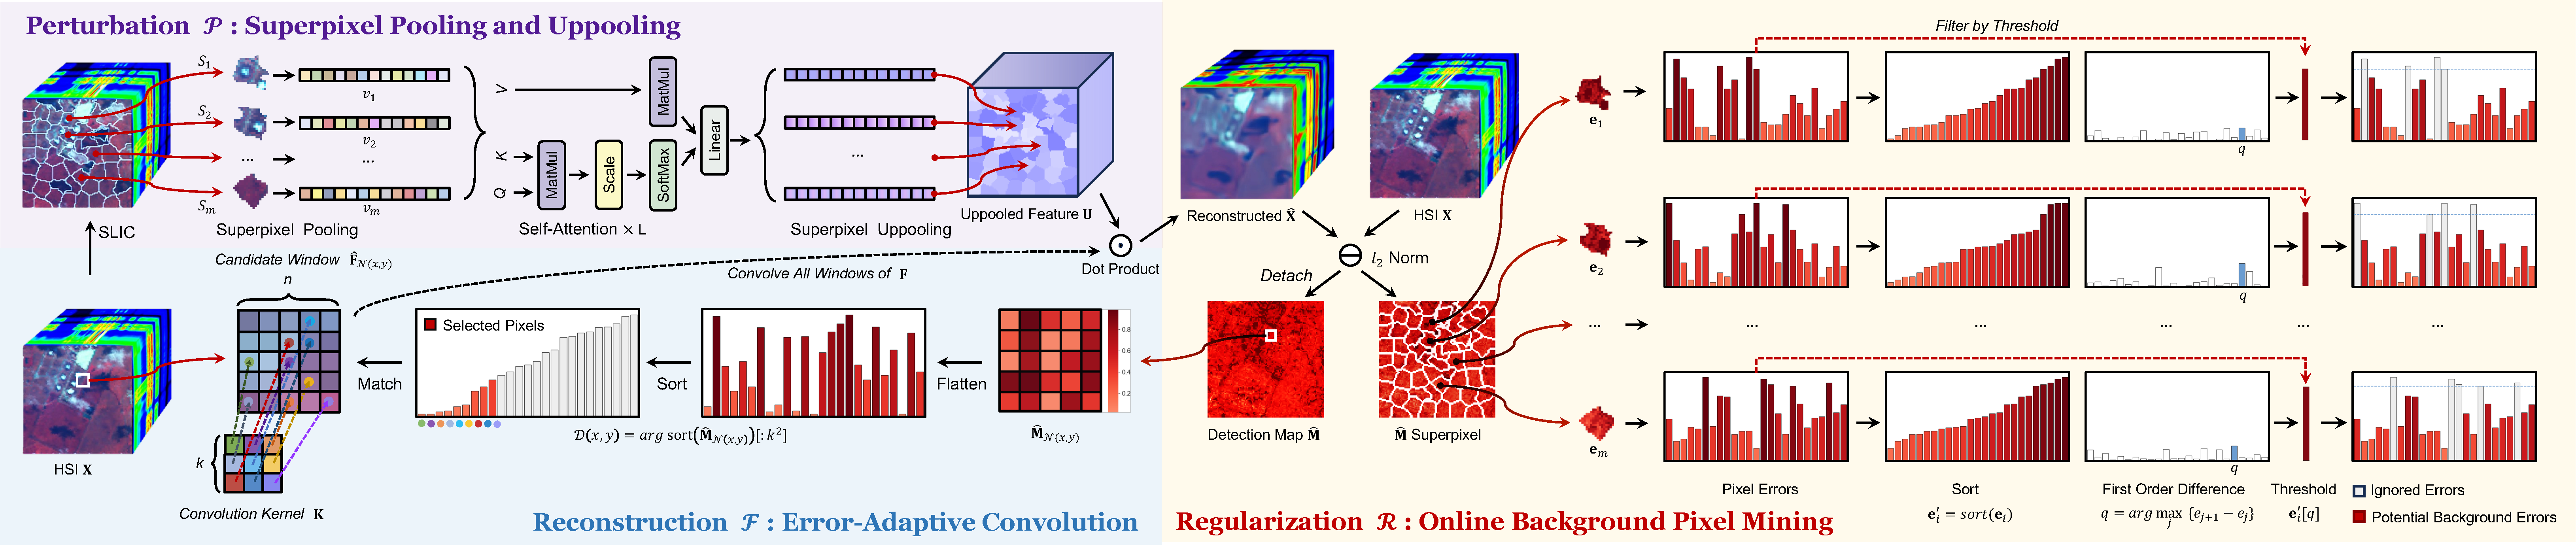
\includegraphics[width=1\linewidth]{net.pdf}
    \caption{Our proposed unified framework for self-supervised HAD (Zoom in for better view), including the perturbation operation $\mathcal{P}(\cdot)$, the reconstruction function $\mathcal{F}(\cdot,\cdot;\theta)$, and the regularization term $\mathcal{R}(\cdot)$. For every part, we propose the corresponding solution to address the IMP, including the superpixel pooling and unpooling (SPP), error-adaptive convolution (AdaConv), and online background pixel mining (OBPM).} \label{fig:net}
  \end{figure*}

\subsection{Deep Learning-based Self-Supervised Methods}

Linear assumptions of traditional statistical methods and shallow feature extraction mechanisms make it difficult to fully explore the nonlinear associations and deep semantic information implied in HSI data. Deep learning excels in in nonlinear feature extraction, which has been extensively employed in HSI anomaly detection with demonstrated effectiveness~\cite{xu2022hyperspectral,xie2020autoencoder,Cui2025Pansharpening,sun2025decadedeeplearningremote}. Autoencoders (AEs)~\cite{zhang2016crop} and Generative Adversarial Networks (GANs)~\cite{jiang2020discriminative} form the main approaches of unsupervised deep learning.

On benchmark datasets, early research by Taghipour et al. showed that simple AE designs with $l_2$ reconstruction loss minimization achieve comparable performance, follow-up studies have shown that deepening the network reduce reconstruction error gaps between anomalous and background pixels, which is explained by the network's tendency to learn uncommon anomaly patterns thanks to its enhanced modeling capacity~\cite{taghipour2019unsupervised,wang2023digging,hartley2004minimization,Cui2024Reconstruction}. The emergence of GANs has provided a new approach to HAD: realistic backgrounds are generated using a training generator, and the discriminator recognizes the anomalies. Wang et al.~\cite{wang2023frequency} used this technique which demonstrated superior separability to achieve a significant improvement in anomaly separability compared to a self-encoder baseline~\cite{goodfellow2014generative,arjovsky2017wasserstein,xu2022hyperspectral,abuhani2025generative,Cui2024Pixel}. In GAN-based techniques, a discriminator locates the anomalies by detecting differences, while a generator is trained to create realistic background pixels. By integrating GAN adversarial training with AE reconstruction, AAE~\cite{xie2020autoencoder} limits the latent space distribution. HAD has recently seen major improvements with the advent of Transformer architectures. For instance, Transformers like SpectralFormer~\cite{wu2024transformer} represent global spectrum dependencies using a self-attentive method, achieving top results anomaly detection capabilities on benchmark hyperspectral datasets. However, the computational cost of these methods is greatly increased by their effectiveness~\cite{liu2024msnet}. This is why masked autoencoding techniques~\cite{vaswani2017attention} randomly exclude most spectral bands during training in an effort to strike a balance between performance and efficiency. Exploiting inter-band correlations has proven to have significant limitations in real-world deployments, despite its effectiveness in controlled trials~\cite{zhang2023spectrum}, particularly when working with data from innovative sensor systems.

Despite the recent advancements in HAD, identity mapping problem (IMP) related flaws are still present in current approaches. The IMP stems from the network's memorize anomaly patterns. First, over-parameterization is directly related to IMP susceptibility, with over-parameterized networks showing higher vulnerability~\cite{mou2017deep,luo2022frequency}. Second, IMP happens regardless of architectural changes, and the global reconstruction aim basically pushes the network in the direction of identity mapping. Third, anomalies can be accurately reconstructed from surrounding band information thanks to strong spectral correlation~\cite{li2024superpixel}. Let $\mathcal{F}$ be the neural network and $X$ be the input HSI of a self-supervised model (\textit{e.g.,} AE). When $\mathcal{F}(\mathbf{X}) \approx \mathbf{X}$ holds for every pixel, including anomalies, IMP takes place. The reconstruction error $\|\mathbf{X} - \mathcal{F}(\mathbf{X})\|$, which goes to zero and loses discriminative qualities, is what anomaly detection depends on. In this instance, the model's ability to distinguish normal and abnormal pixels is compromised, which lowers the efficacy of anomaly detection. The error of abnormal pixels that appear as unnoticeable abnormal pixels increases in HAD as the network complexity~\cite{chang2020effective} or the number of training iterations and the accurate reconstruction of anomalies grow. The more complex or well-trained the model, the more likely it is to learn the identity mapping ($\hat{X} \approx X$) that includes anomalies and background, rather than extracting discriminative features. 
